% !TEX TS-program = XeLaTeX 
% Commands for running this example:
% xelatex picinpar-example
% End of Commands
\documentclass{article}
\pagestyle{empty}
\usepackage{picinpar,graphicx}
\usepackage{xepersian}
\begin{document}
\begin{figwindow}[3,r,%
 \fbox{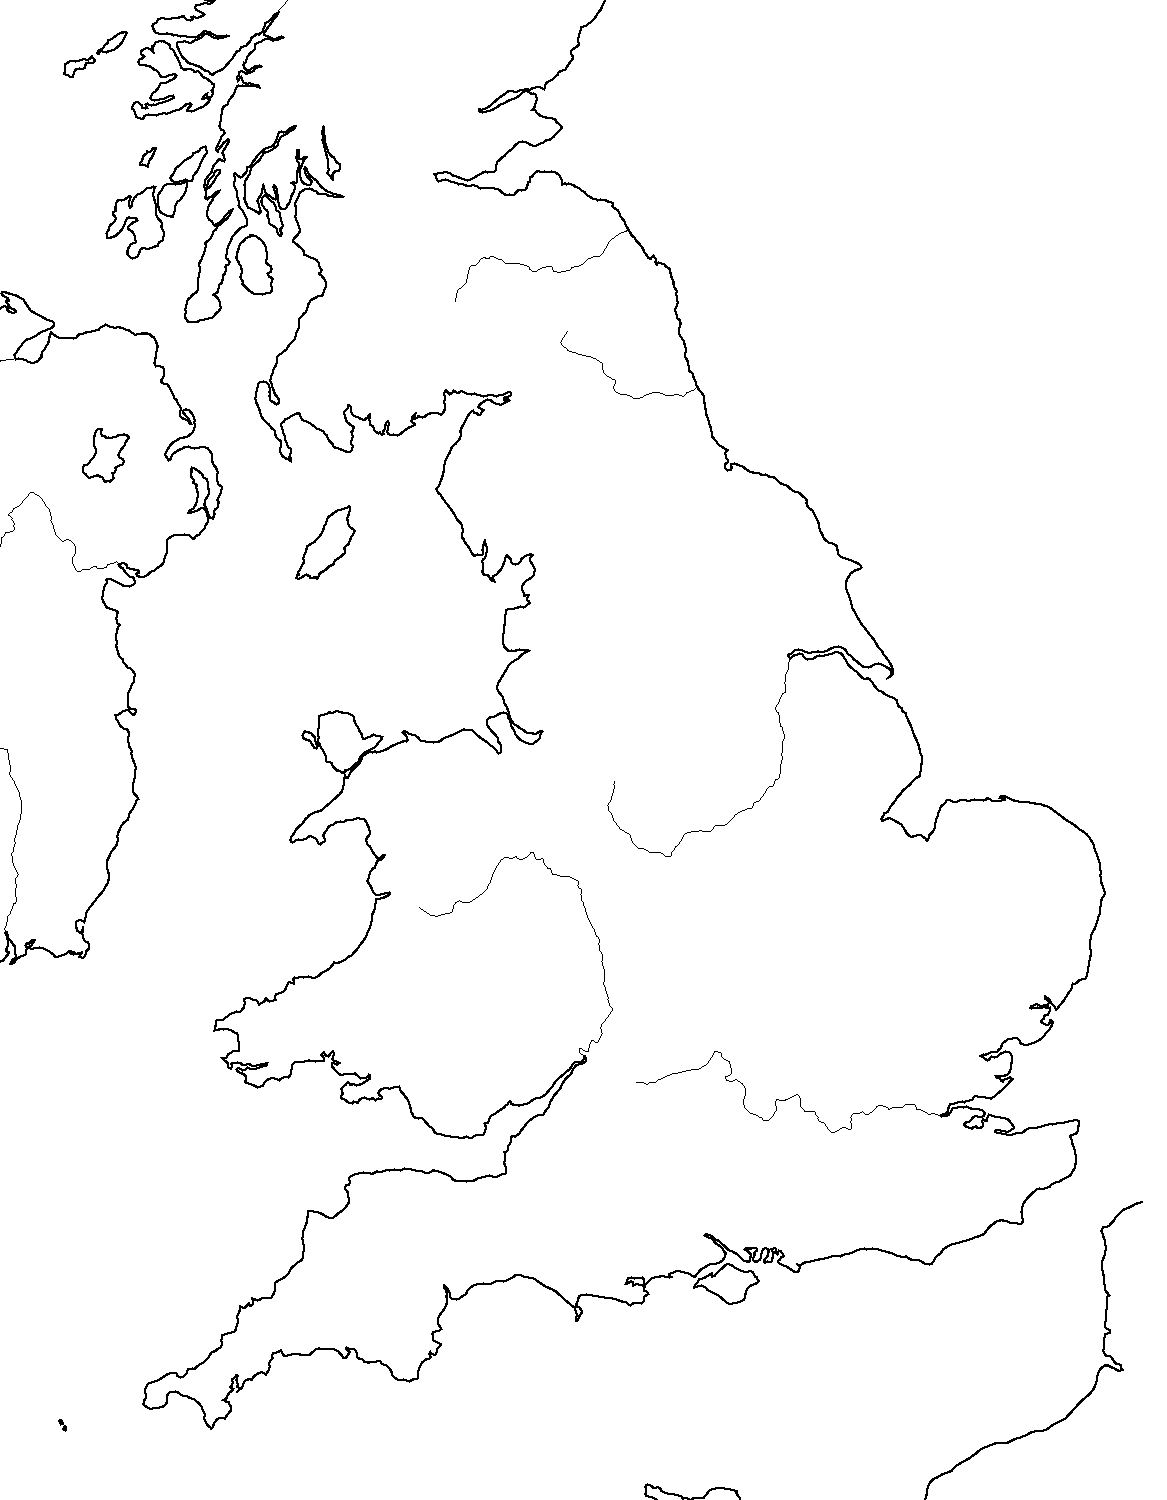
\includegraphics[width=30mm]{map}},%
                  {این یک نقشه است.}]
جغرافی‌دانان به گونه‌ای سنتی، عده‌ای نقشه‌نگار که به بررسی نام مکان‌ها و تعدادشان می‌پردازند، به نظر می‌رسند. اگر چه بسیاری از جغرافی‌دانان در مکان‌نامی(ذکر نام‌های نواحی) و نقشه‌نگاری آموزش دیده‌اند، ولی‌این کار پیشهٔ اصلی‌شان نیست. جغرافی‌دانان به بررسی پراکندگی مکانی و زمانی پدیده‌ها، فرآیندها، ویژگی‌ها و هم‌چنین برهم‌کنش انسان و محیط زیست او به عنوان اثر فضا و مکانِ تحت تأثیر موضوعات مختلف از جمله اقتصاد، بهداشت، آب و هوا، گیاهان و جانوران، می‌پردازند؛ از این رو جغرافیا دانشی میان‌رشته‌ای و فرارشته‌ای است.
جغرافیا در یک چینش می‌تواند به طور گسترده به دو شعبهٔ اصلی تقسیم شود: جغرافیای انسانی و جغرافیای فیزیکی. اولی تا حد زیادی بر معماری و چگونگی‌ایجاد فضا متمرکز است -که با انسان مشاهده و مدیریت می‌شود و نیز نفوذ او فضا و مکان به خاطر به‌کارگیری و چنگ‌اندازی‌اش به آن می‌فرساید. دومی به بررسی محیط زیست طبیعی و چگونگی به وجود آمدن و تداخل آب‌وهوا، پوشش گیاهی و چرخهٔ زیستی، خاک، آب، و زمین‌چهره می‌پردازد. به عنوان برآیندی از این دو زیرحوزه و با استفاده از روش‌های متفاوت، حوزهٔ سومی پدید آمده‌است که جغرافیای زیست‌محیطی نام دارد.
\end{figwindow}
\end{document}
